\documentclass[10pt]{beamer}

\usetheme[progressbar=frametitle]{metropolis}
\usepackage{appendixnumberbeamer}

\usepackage{booktabs}
\usepackage[scale=2]{ccicons}

\usepackage{pgfplots}
\usepgfplotslibrary{dateplot}

\usepackage{xspace}
\newcommand{\themename}{\textbf{\textsc{metropolis}}\xspace}

\usepackage{multimedia}
\usepackage{hyperref}
\usepackage{subcaption}
\usepackage{tikz}

\graphicspath{ {figures/} }

\title{Tesselated Voxelization for Global Illumination using Voxel Cone Tracing}
%\subtitle{}
\date{June 2018}
\author{Sam Freed\\\\Committee Members:\\ Dr.\ Christian Eckhardt (chair), Dr.\ Maria Pantoja, Dr.\ Aaron Keen\\}
\institute{California Polytechnic State University, San Luis Obispo}
% \titlegraphic{\hfill\includegraphics[height=1.5cm]{logo.pdf}}

\AtBeginSection[]
{
	\begin{frame}
    	\frametitle{Outline}
        \tableofcontents[currentsection,hideothersubsections] % TODO show subsections/frames?
	\end{frame}
}

\begin{document}

\frame{\titlepage}

% Go over outlines of presentation. Mention the subsections briefly as appropriate.
\begin{frame}{Outline}
  \setbeamertemplate{section in toc}[sections numbered]
  \tableofcontents[hideallsubsections]
\end{frame}

\setbeamertemplate{frametitle continuation}{}

\section{Introduction}

\begin{frame}{Introduction}
% who i am, thanks for coming, blah blah

% what is global illumination and why important
% show AO and baked? or at least talk about it and show pictures
% we want FULL GI
  \begin{block}{Computer Graphics}
    How can we model light in a virtual world?

    Physically accurate lighting too complex for real-time---approximate!
  \end{block}
\end{frame}

\begin{frame}{Computer Graphics}
  % here we only have simple lighting. the ambient/indirect light is the difficult part to compute

  % Want to go from this...to _this_
  % \begin{columns}
  %   \begin{column}{0.5\textwidth}
      \begin{figure}
        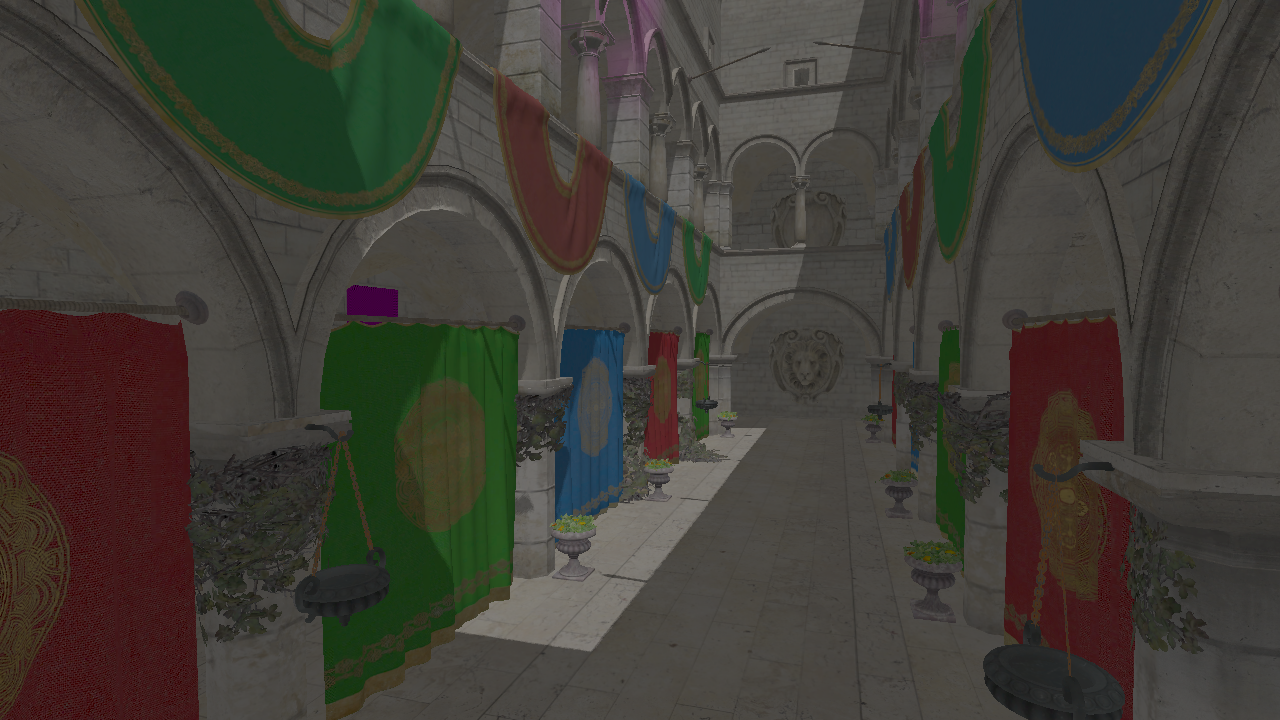
\includegraphics[width=\textwidth]{gi_off.png}
        :(
      \end{figure}
    \end{frame} \begin{frame}{Motivations}
  %   \end{column}
  %   \begin{column}{0.5\textwidth}
      \begin{figure}
        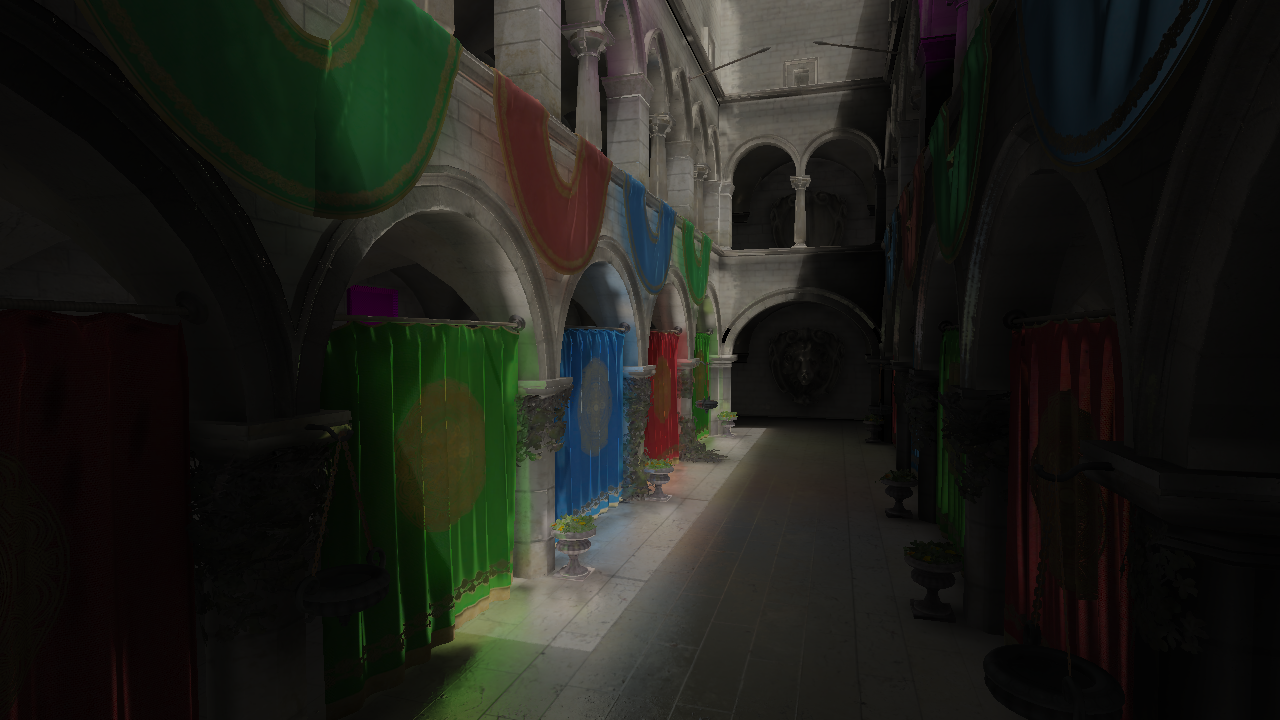
\includegraphics[width=\textwidth]{gi_on.png}
        :)
      \end{figure}
  %   \end{column}
  % \end{columns}
\end{frame}

\begin{frame}{Real-Time Global Illumination}
  Various approaches to approximating indirect light.

  \begin{description}
    \item[Constant] Fixed fraction of ambient light % as seen in first image
    \item[Partial] Ambient occlusion, shadows, screen space reflections % only model parts of global illumination; often local methods that do not have complete scene information
    \item[Static] Baked lighting
    \item[Dynamic] Light Propagation Volumes, Voxel Cone Tracing
  \end{description}
\end{frame}

% \begin{frame}{Teaser}
% % video or screenshots, show good lighting + moving objects
% \movie[autostart,showcontrols]{\textcolor{black}{\rule{\textwidth}{0.9\textheight}}}{test.webm}
% \end{frame}

% \begin{frame}{What did I just see?}
% % real time gi of course!
% \end{frame}

\subsection{Motivations}
\begin{frame}{Motivations}
  \begin{enumerate}
    \centering
    \item Real-time global illumination is difficult % lots of computation
    \item Limited reference material % open-source, cross-platform (-apple), no large engine, any documentation or explanation
    \pause
    \item I think it's cool % the real reason tbh
  \end{enumerate}
\end{frame}

\subsection{Contributions}
\begin{frame}{Contributions}
  \begin{itemize}
    \item Open-source, cross-platform implementation of global illumination using voxel cone tracing
    \item Comparison between rasterization and tessellation based voxelization
    \item Investigation into warped voxels % more on this later, first I'd like to give a crash course in graphics and an overview of other solutions to real time gi
  \end{itemize}
\end{frame}


\section{Background}

\subsection{Computer Graphics}
\begin{frame}{Computer Graphics Primer}
  \begin{block}{Goal}
    Given a virtual description of a scene render an image.
  \end{block}

  \begin{block}{Big Issues}
    \begin{enumerate}
      \item How do we represent a scene? What information is required?  % geometry (triangles, voxels), materials (colors, properties), lights (type, position, color, direction), etc.
      \item How is a 3D scene represented as a 2D image?  % implies some transformation needed
      \item How do we `render'---how is the final pixel color computed? % lighting/shading model; this is the focus of this thesis
    \end{enumerate}
  \end{block}
  % rtr objects -> world space -> screen space
  % goal of computer graphics; graphics pipeline; transforms and other common stuff
\end{frame}

\begin{frame}{How do we represent a scene?}
  \setbeamercovered{transparent}
  \begin{columns}
    \begin{column}{0.5\textwidth}
      \begin{itemize}[<+>]
        \item Geometry: triangles, voxels % triangles inherently 2D->good for surfaces, not so much for volumetric data
        \item Materials: colors and other properties % like roughness, normal maps (kinda)
        \item Lights: positions, colors, etc.
      \end{itemize}
    \end{column}
    \begin{column}{0.5\textwidth}
      \only<1>{
        \begin{figure}
          \begin{subfigure}{\textwidth}
            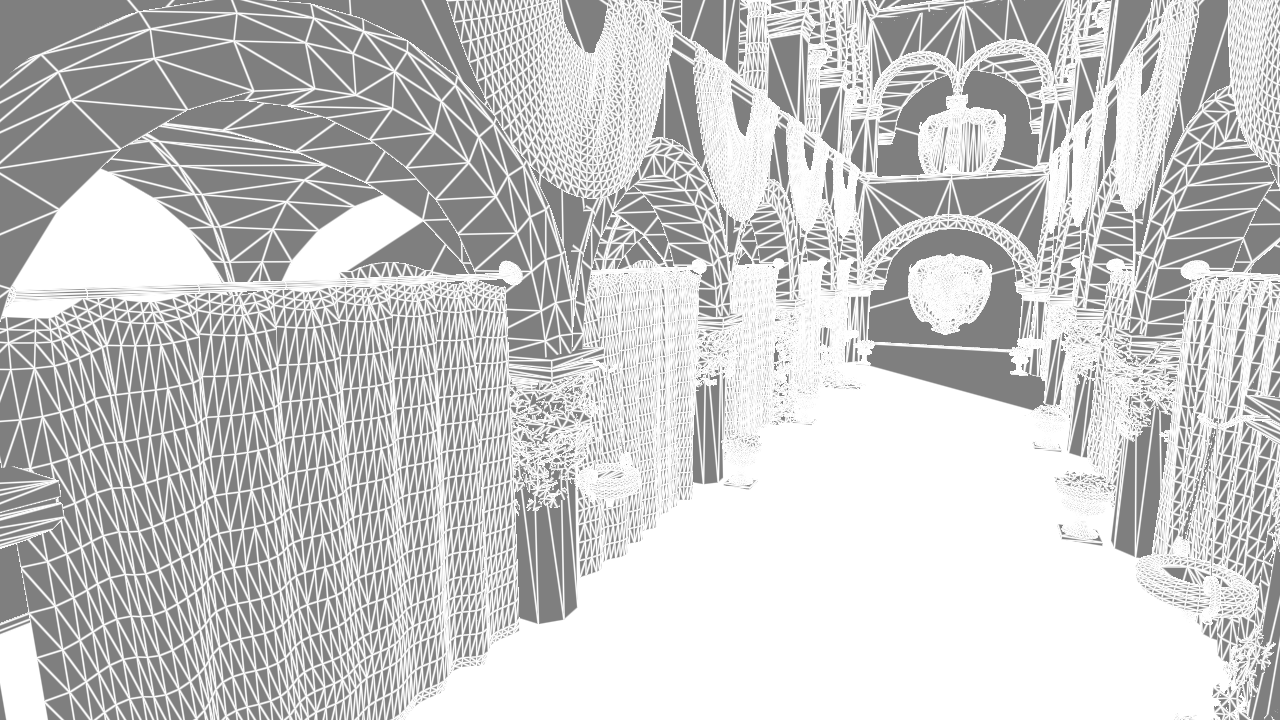
\includegraphics[width=\textwidth]{wireframe.png}
          \end{subfigure}
          \begin{subfigure}{\textwidth}
            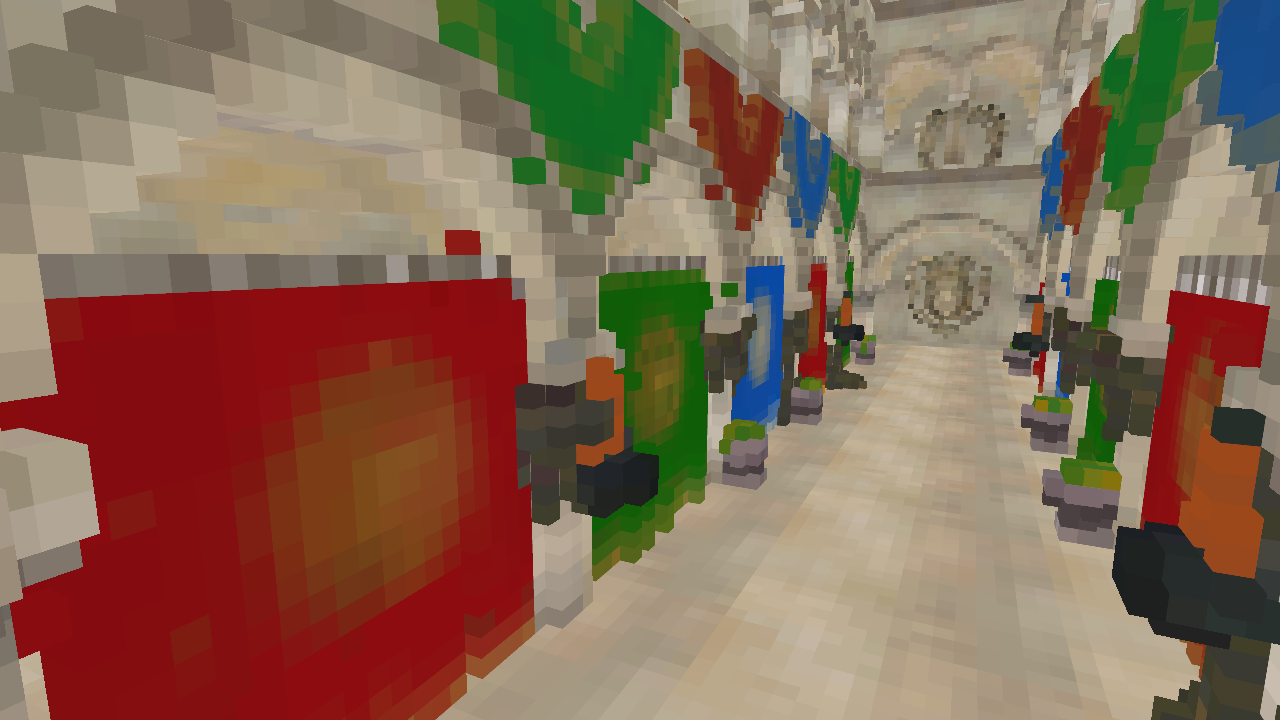
\includegraphics[width=\textwidth]{voxels.png}
          \end{subfigure}
        \end{figure}}

      \only<2>{
        \begin{figure}
          \begin{subfigure}{\textwidth}
            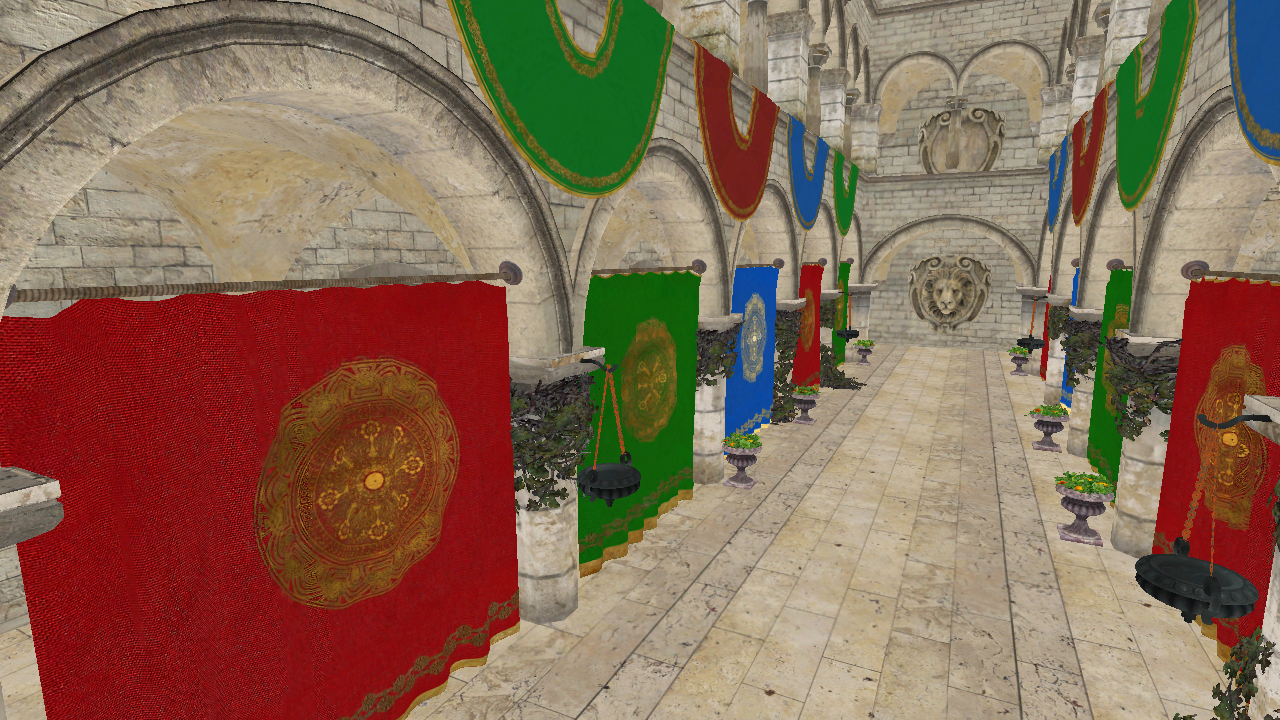
\includegraphics[width=\textwidth]{albedo.png}
          \end{subfigure}
          \begin{subfigure}{\textwidth}
            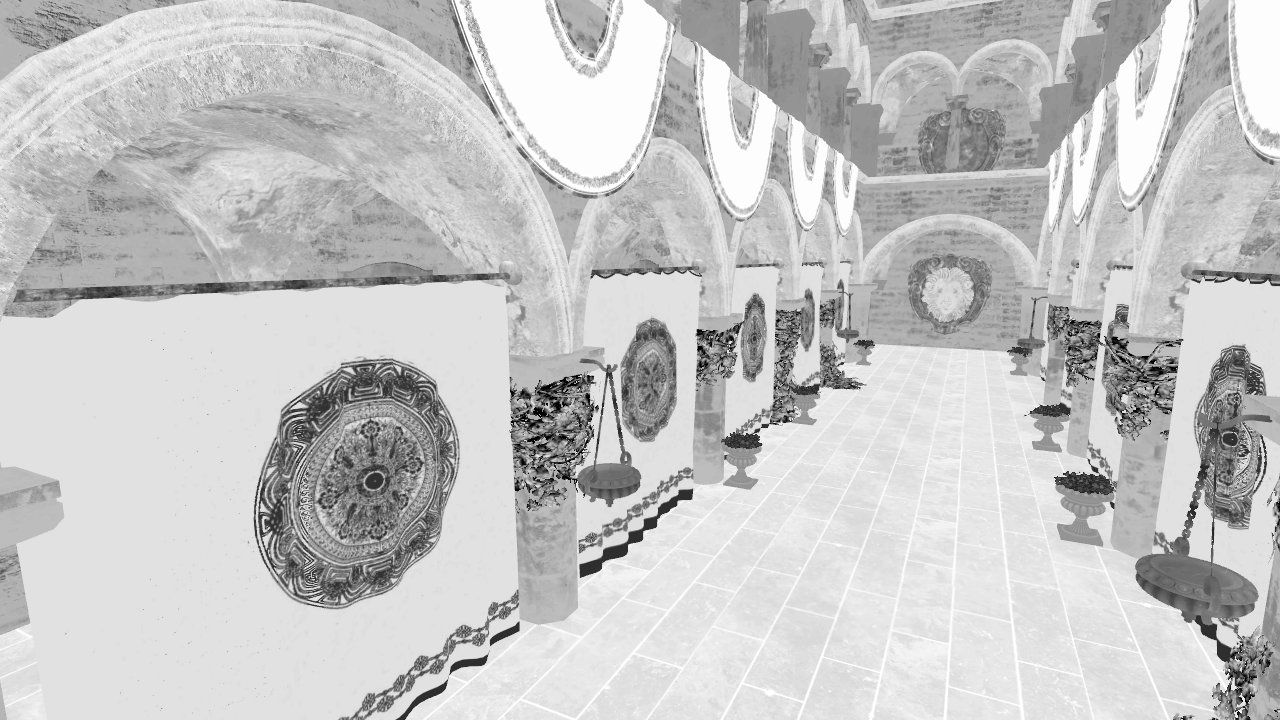
\includegraphics[width=\textwidth]{roughness.png}
          \end{subfigure}
        \end{figure}}

      \only<3>{
        \begin{figure}
          \begin{subfigure}{\textwidth}
            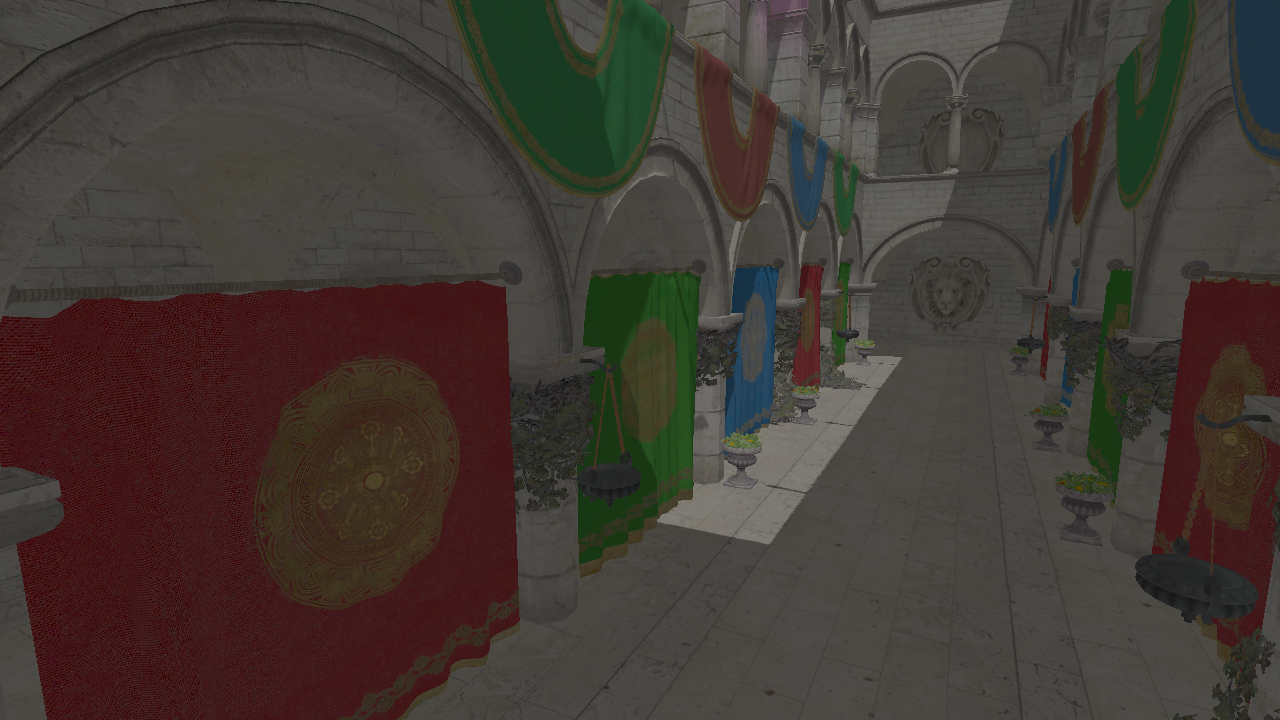
\includegraphics[width=\textwidth]{nogi.png}
          \end{subfigure}
          \begin{subfigure}{\textwidth}
            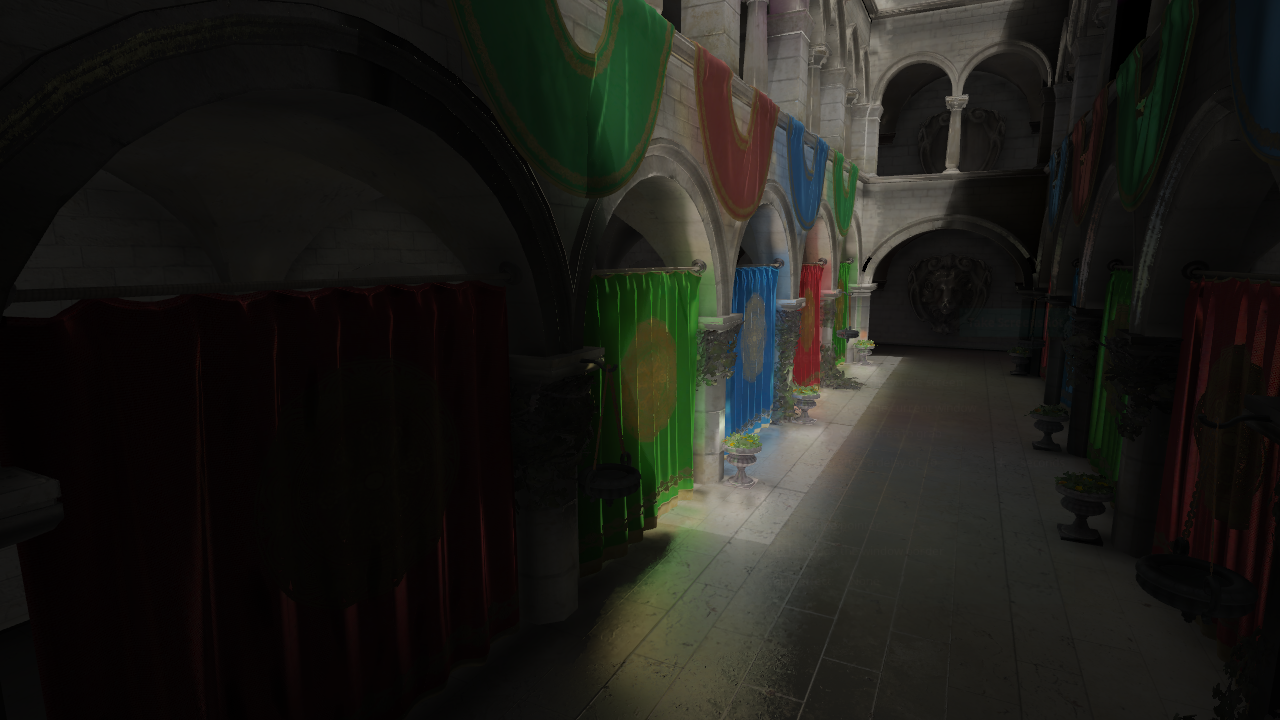
\includegraphics[width=\textwidth]{gi.png}
          \end{subfigure}
        \end{figure}}
    \end{column}
  \end{columns}
\end{frame}

{\setbeamertemplate{frame footer}{image from Real-Time Rendering} % TODO cite
\begin{frame}{How is a 3D scene represented as a 2D image?}
  Math!

  All coordinates are transformed multiple times before ending up at their appropriate place on the screen.

  \begin{figure}
    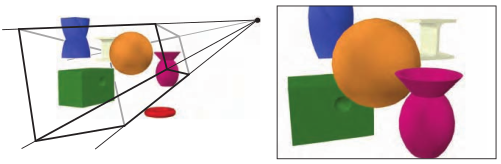
\includegraphics[width=\textwidth]{rtr_fig2_1.png}
  \end{figure}

\end{frame}}


\begin{frame}{How is a 3D scene represented as a 2D image?}
  % picture of coordinate systems and give brief explanation, since explain more along with the graphics pipeline
  % showing this so everyone is comfortable when explaining algorithms
  % ...and this is accomplished with <flick> THE GRAPHICS PIPELIIIIIIINE

  \begin{figure}
    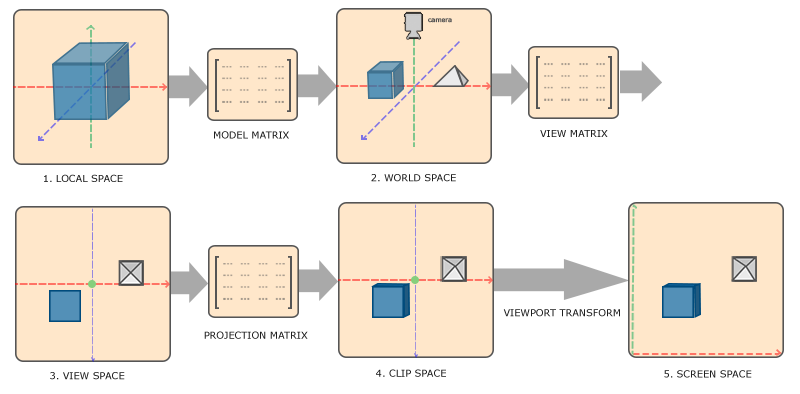
\includegraphics[width=\textwidth]{learnopengl_coordinate_systems.png}
  \end{figure}

  \begin{description}[<+| only@+>]
    \item[Local/Object Space] coordinate system relative to a single object
    \item[World Space] a global coordinate system for the virtual world
    \item[View Space] coordinates are with respect to the camera
    \item[Clip Space/NDC] defines a frustum in which objects will be rasterized % those outside the frustum are clipped
    \item[Screen Space] coordinates are the pixel position and a depth value
  \end{description}

  % Also other spaces, like texture space [0, 1], image space (integral coordinates),

\end{frame}

\begin{frame}{How is a 3D scene represented as a 2D image?}
  \begin{center}
    \huge\textbf{The Graphics Pipeline}
  \end{center}
  % picture of pipeline
  % This is the standard sequence of events that render the final image from our scene
  % We'll go over the entire pipeline for sake of completess
  \begin{figure}
    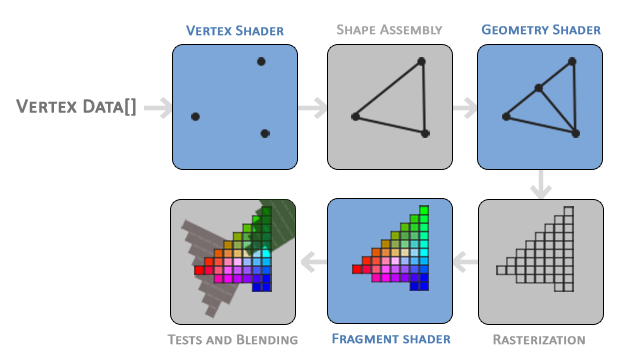
\includegraphics[width=\textwidth]{learnopengl_graphicspipeline.png}
  \end{figure}
\end{frame}

\begin{frame}{The Graphics Pipeline}
  \begin{figure}
    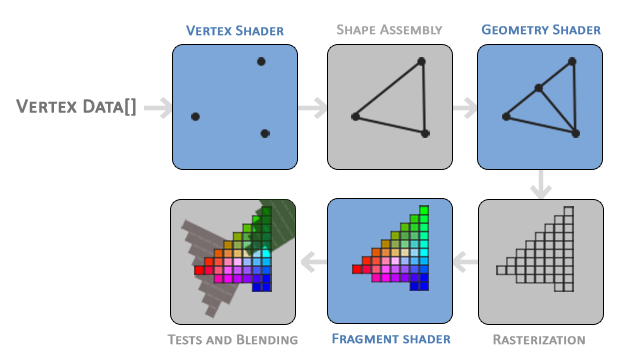
\includegraphics[width=\textwidth]{learnopengl_graphicspipeline.png}
  \end{figure}

  \begin{description}[<+| only@+>]
    \item[Input] A series of vertices containing attributes like position, normal, and texture coordinates
    \item[Vertex Shading]
    \item[Shape Assembly]
    \item[Geometry Shading]
    \item[Rasterization]
    \item[Fragment Shading]
    \item[Testing and Blending]
  \end{description}
\end{frame}

\begin{frame}{Compute Shader}
  % just want to introduce the concept since I'll mention them in implementation
\end{frame}

% \begin{frame}{Tessellation}
%   % briefly go over triangle tessellation and where it fits in the pipeline. will probably talk about it more in implementation

%   \begin{figure}
%     
\includegraphics[height=\textheight]{openglwiki_tesselation.png}
%   \end{figure}
% \end{frame}

\begin{frame}{Spatial Data Structures}
  % quickly go through one slide each (with picture)
  \begin{description}
    \item<1>[Uniform Texture] each cell is the same size  % simple, hw filtering; wasteful
    \item<2>[Cascaded Texture/Clipmap] nested textures with varying cell sizes % there is difference but not important for us; cell sizes are discrete multiplies, still wasteful but better, need to handle edges properly
    \item<3>[Octree] adaptive tree structure which holds values in leaves % sparse, difficult on gpu to build and traverse, no hw filtering
  \end{description}

  \begin{figure}
    % TODO TODO TODO \includegraphics<+>[width=\textwidth]{}
    \only<1>{
\begin{tikzpicture}[scale=0.8]
      \draw [black, step=1.0] (-4, -4) grid ++(8, 8);
    \end{tikzpicture}}
    % \includegraphics<+>[width=\textwidth]{geometry_clipmap.jpg}
    \only<2>{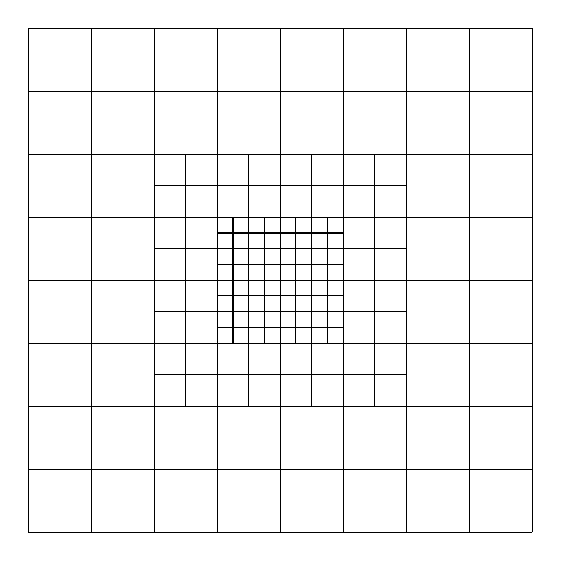
\begin{tikzpicture}[scale=0.8]
      \draw [black, step=1.0] (-4, -4) grid ++(8, 8);
      \draw [black, step=0.5] (-2, -2) grid ++(4, 4);
      \draw [black, step=0.25] (-1, -1) grid ++(2, 2);
    \end{tikzpicture}}
    % \includegraphics<3>[width=\textwidth]{octree.png}
    \only<3>{\begin{tikzpicture}[scale=0.8]
      \draw [black, step=4.0] (-4, -4) grid ++(8, 8);
      \draw [black, step=2.0] (0, 0) grid ++(4, 4);
      \draw [black, step=1.0] (2, 2) grid ++(2, 2);
      \draw [black, step=1.0] (2, 0) grid ++(2, 2);
      \draw [black, step=0.5] (2, 1) grid ++(1, 2);
      \draw [black, step=0.25] (2, 1.5) grid ++(1, 1);
    \end{tikzpicture}}
  \end{figure}
\end{frame}

\begin{frame}{How do we `render'?}
  % We need a shading model: a way to compute a color from the geometry, lights, and materials we have in the scene for a particular point
  % Makes sense to model this based on the real-world sooo
  % See the next section!
\end{frame}

\subsection{Lighting}
\begin{frame}{Radiance and the Rendering Equation}
  % Semi-detailed, need to have audience at least have some idea what's going on
  % Note how this is computationally intensive -> need to resort to approximations
\end{frame}

\begin{frame}{Direct Lighting}
  % use as example of how lighting works, some intuition on rendering equation
  % should help to understand indirect lighting
\end{frame}

\begin{frame}{Indirect Lighting}
  % what is is, other approaches, general approaches?
\end{frame}

% raytracing and raymarching? maybe one slide

% ask for any questions or clarification here? (after related work too maybe?)

\section{Related Work}

\subsection{VPLs and RSMs}
\begin{frame}{VPLs and RSMs}
  % Just want to introduce the concept of VPLs and RSMs are simple way of doing that
  \begin{description}
    \item[Virtual Point Lights] Treat arbitrary objects or locations as light sources
    \item[Reflective Shadow Maps] Treat each pixel of a shadowmap as a VPL % when rendering project point into shadowmap and gather lighting contributions from VPLs; problem is poor occlusion information and only low frequency lighting
  \end{description}

  \begin{figure}
    \includegraphics<+>[width=\textwidth]{rsm.png}
    \includegraphics<+>[width=\textwidth]{rsm_vpl.png}
  \end{figure}

  % another slide for pros/cons?
\end{frame}

\subsection{Light Propagation Volumes}
\begin{frame}{Light Propagation Volumes}
  % low frequency but fairly stable, no occlusion (limited info from reusing), cascaded
  % iterative process to propagate light throughout scene

  \begin{itemize}
    \item Store VPLs in a voxel grid
    \item Iteratively propagate lighting contribution until stable
  \end{itemize}

  \begin{figure}
    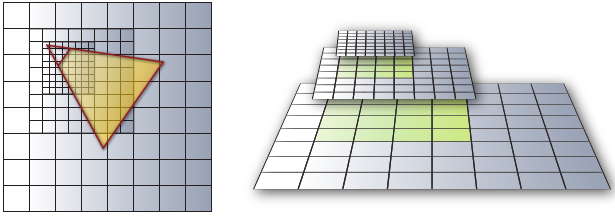
\includegraphics[width=\textwidth]{lpv.png}
  \end{figure}
\end{frame}

\subsection{Voxel Cone Tracing}
\begin{frame}{Voxel Cone Tracing}
  % complete occlusion info, sparse voxel octree, specular reflections

  \begin{itemize}
    \item Sparse voxel octree % occlusion information
    \item High resolution (diffuse and specular lighting)
  \end{itemize}

  \begin{figure}
    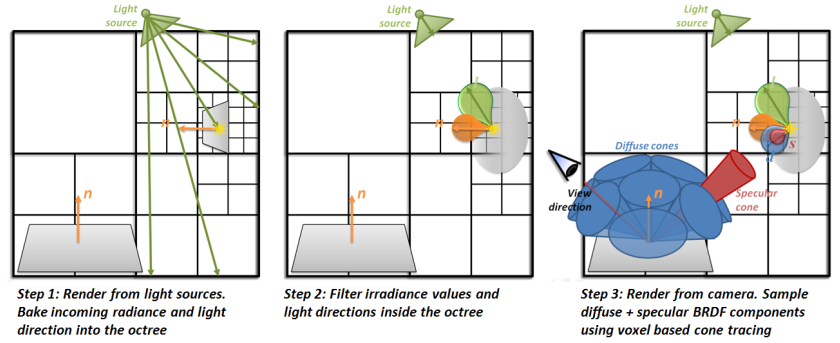
\includegraphics[width=\textwidth]{vct.png}
  \end{figure}
\end{frame}

% TODO quick recap here?
% most important bits: voxels represent 3d data well and thus voxelization is important; vpls are core part of most gi algorithms; lpv and vct use regular grid

\begin{frame}{What am I doing?} % this is the research question
  \begin{enumerate}
    \item Comparing two approaches for scene voxelization % voxelization is a core part of the algorithm; tessellated version also not restricted to rasterizer
    \item Investigating continuous voxel sizes % voxel warping; idea is to support bigger scenes and increase resolution near camera without abrupt changes in voxel density
  \end{enumerate}
\end{frame}

\section{Implementation}

\begin{frame}{Overview of Renderer}
  % flowchart or something showing each render pass
  % list of all major resources (3ish voxel textures, shadowmap, meshes, materials)

  \begin{columns}
    \begin{column}{0.5\textwidth}
      \begin{block}{Main Steps}
        \begin{enumerate}
          \item Setup (load scene, create textures, compile shaders)
          \item Create Shadowmap
          \item Voxelize Scene
          \item Inject Radiance
          \item Filter Radiance
          \item Depth Prepass
          \item Shading
        \end{enumerate}
      \end{block}
    \end{column}
    \begin{column}{0.5\textwidth}
      \begin{block}{Important Data}
        \begin{enumerate}
          \item Scene (meshes, materials, lights)
          \item Camera (position, direction) %, projection + view matrices)
          \item Shadowmap % Framebuffer Object and Texture
          \item Voxel Textures (color + opacity, normals, radiance)
        \end{enumerate}
      \end{block}
    \end{column}
  \end{columns}
\end{frame}

\subsection{Voxelization}
\begin{frame}{Voxelization with Rasterizer}
  Each fragment corresponds to a voxel
  % main idea: rasterized fragments correspond to voxel
  % setup: need projection matrices
  % geometry shader: choose dominant axis and project
  % fragment shader:

  \begin{figure}
    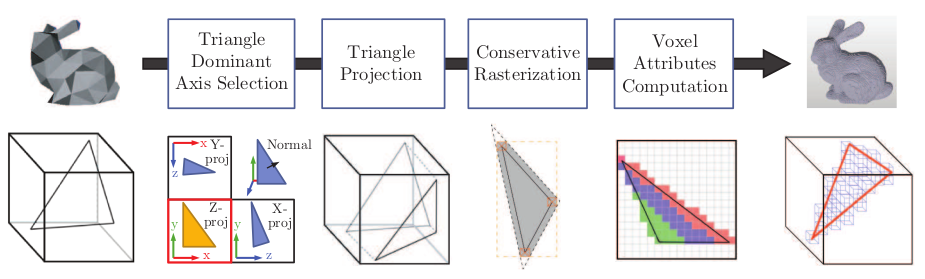
\includegraphics[width=\textwidth]{rasterizedvoxelization}
  \end{figure}
\end{frame}

\begin{frame}{Voxelization with Tessellator}
  Idea: Generate a \textit{vertex} for each voxel instead of a fragment

  % Tessellation after vertex shading and before fragment shading
  % rasterizer is not needed (is disabled)
  % don't need to worry about dominant axis or conservative rasterization

  \begin{figure}
    
\includegraphics[scale=0.8]{openglwiki_tesselation.png}
  \end{figure}
\end{frame}

\begin{frame}{Determining Tessellation Levels}
  Outer levels determined from respective edge lengths

  Inner level determined from maximum triangle altitude length

  % TODO triangle overlaid on grid with tessellated points?
\end{frame}

\begin{frame}{Voxelized Scene}
  \begin{figure}
    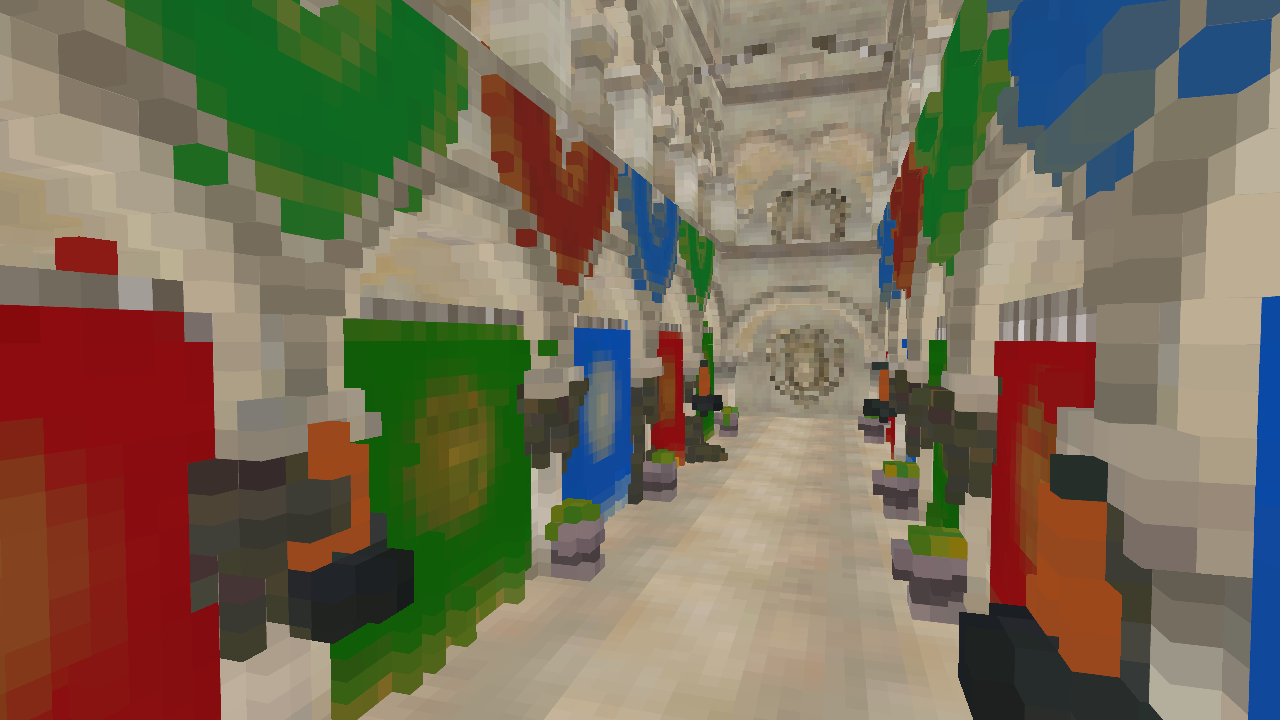
\includegraphics[width=\textwidth]{voxels_msaa}
  \end{figure}
\end{frame}

\subsection{Radiance Injection and Filtering}
\begin{frame}{Radiance Injection}
  \begin{itemize}
    \item Create virtual point lights for all geometry hit by the light.
    \item These lights approximate a single-bounce of indirect lighting.
  \end{itemize}

  \begin{figure}
    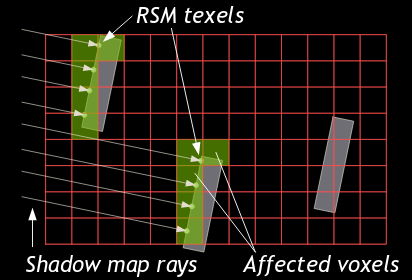
\includegraphics[width=0.8\textwidth]{lightinjection}
  \end{figure}
\end{frame}

\begin{frame}{Radiance Injection---Shadow Mapping}
  To determine where the virtual point lights should be, we use a \textbf{shadowmap}.

  Render the scene from the \textit{light}'s point of view.

  % Only interested in depth values important for us: along with the light matrix we can reconstruct world positions
  % picture
  % implementation? ortho matrix, projection

  \begin{figure}
    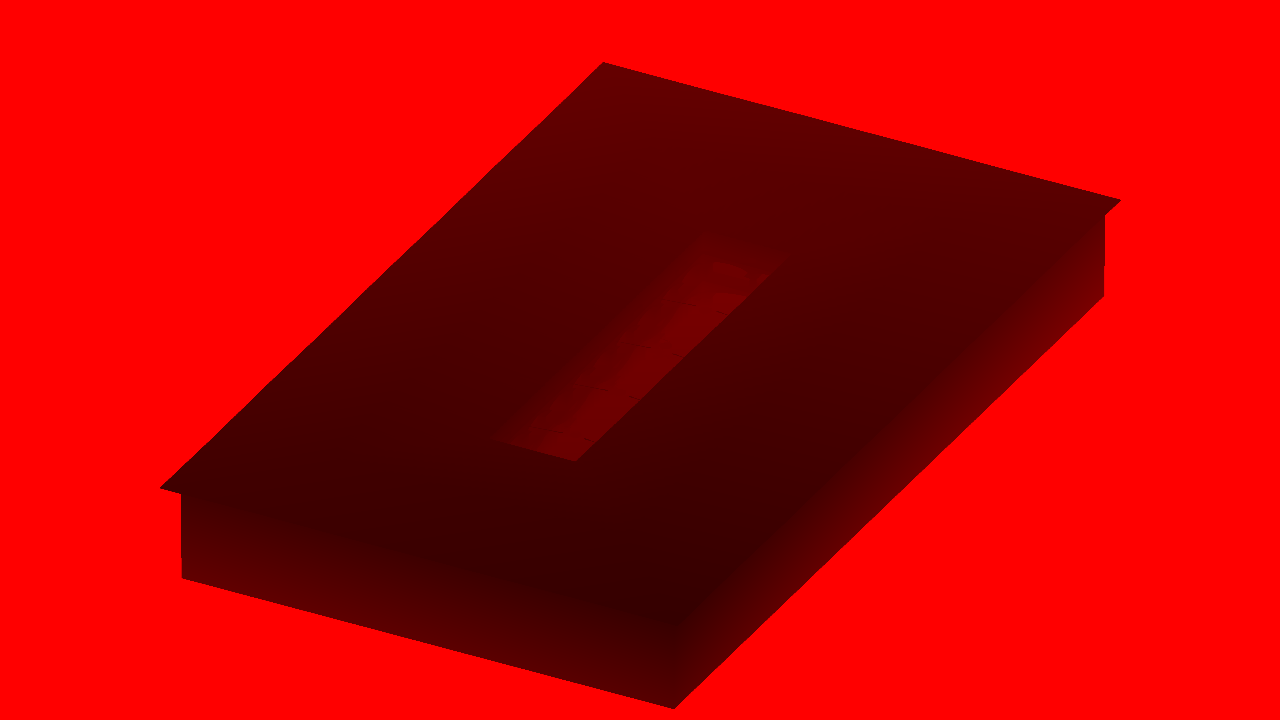
\includegraphics[width=0.8\textwidth]{shadowmap}
  \end{figure}
\end{frame}

\begin{frame}{Radiance Injection---Injecting VPLs}
  For each pixel in the shadowmap, find it's voxel index and insert the corresponding color into the radiance texture.

  Using the light matrix and stored depth value, we compute the point's world space position.

  \begin{figure}
    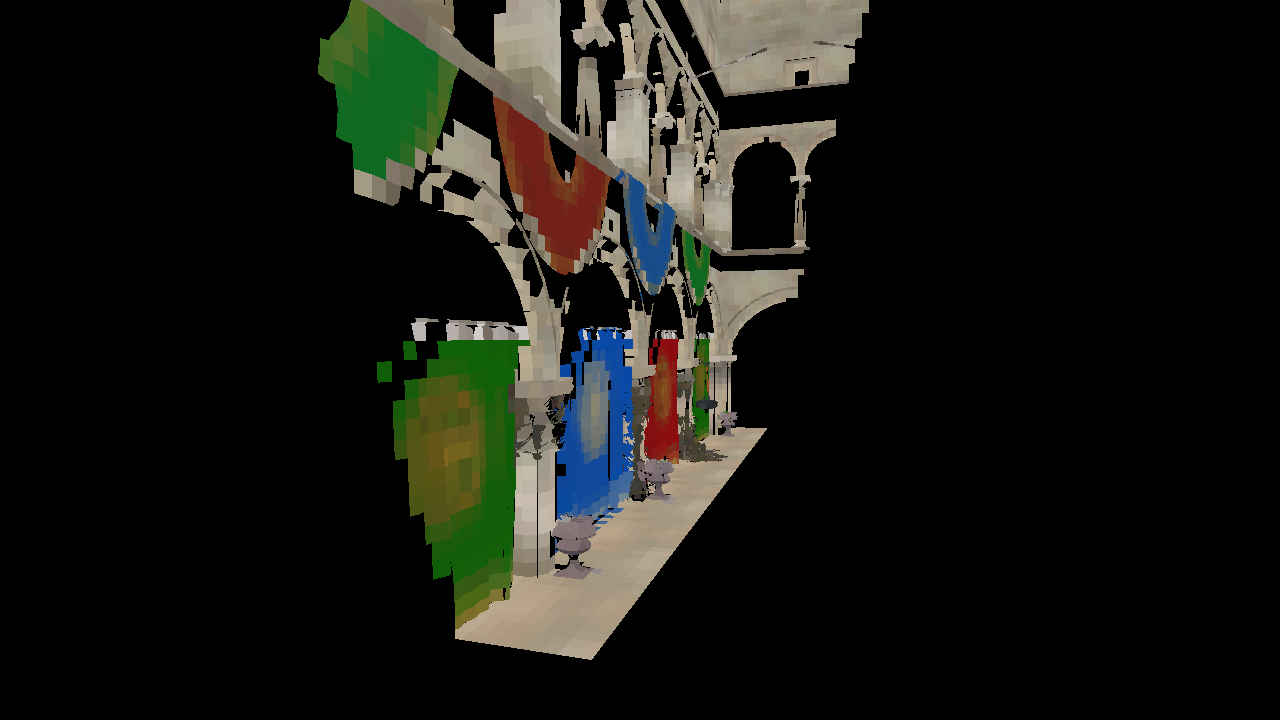
\includegraphics[width=0.8\textwidth]{radiance_nolighting}
  \end{figure}
\end{frame}

\begin{frame}{Radiance Filtering}
  Radiance texture contains multiple \textbf{levels} (mipmaps). Each level is half the size of the previous. A compute shader performs a 2x2x2 box filter for each level to determine the filtered value.

  \begin{center}
    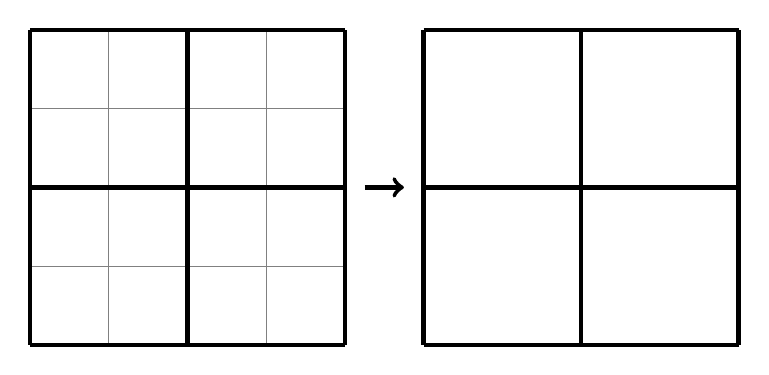
\begin{tikzpicture}
      \draw[step=1.0, gray] (0, 0) grid (4, 4);
      \draw[step=2.0, black, ultra thick] (0, 0) grid (4, 4);
      \draw[black, ->, ultra thick] (4.25, 2) to (4.75, 2);
      \draw[step=2.0, black, ultra thick, xshift=5.0cm] (0, 0) grid (4, 4);
    \end{tikzpicture}
  \end{center}

  % show 2D box filter
  % show the four images
\end{frame}

\begin{frame}{Radiance Filtering}
  \begin{figure}
    \includegraphics<+>[width=\textwidth]{mipmap0.png}
    \includegraphics<+>[width=\textwidth]{mipmap1.png}
    \includegraphics<+>[width=\textwidth]{mipmap2.png}
    \includegraphics<+>[width=\textwidth]{mipmap3.png}
    \caption*{\only<1>{Mipmap level 0}\only<2>{Mipmap level 1}\only<3>{Mipmap level 2}\only<4>{\\Mipmap level 3}}
  \end{figure}
\end{frame}

\subsection{Final Shading}
\begin{frame}{Depth Prepass}
  An optimization to minimize the number of shaded fragments.

  Prefill the depth buffer so lighting (including the relatively expensive voxel cone tracing) will only be performed on the visible fragments of the scene. % remind of depth test and this is only for forward rendering (deferred already does this when creating gbuffer)
\end{frame}

\begin{frame}{Final Shading}
  % outline (direct + diffuse indirect + specular indirect)
  % inputs are lights, material, and fragment (with position, normal, texture coordinates)
\end{frame}

\begin{frame}{Direct Lighting}
  % cook torrance too?
  % don't forget shadows
\end{frame}

\begin{frame}{Indirect Lighting}
% explain voxel cone tracing
% the idea (raymarching + mipmaps), choosing cone angles + dirs, diffuse indirect, specular indirect, cone tracing itself
\end{frame}

\subsection{Voxel Warping}
\begin{frame}{Voxel Warping}
\end{frame}


\section{Results and Conclusions}

% \begin{frame}{Test Setup}
% \end{frame}

% First, and most important, test was to measure the general performance of the algorithm. We also varied the voxel grid resolution and screen resolution to see how it affected performance. Thankfully we meet the 60fps goal for all tested resolutions!
\begin{frame}{Performance}
  % pictures of different voxel grid dimensions
  % graphs of performance times for each
  % analysis (which render passes were affected by what, etc)
\end{frame}

% Next we compared the results of the two voxelization algorithms. Visually, they are practically indistiguishable. Performance-wise the rasterization based approach was slightly faster. We might be able to close the gap with more optimizations. One benefit of the tessellated voxelization is the transformed points are not restricted to the viewport resolution.
\begin{frame}[allowframebreaks]{Rasterized vs. Tessellated Voxels}
  \begin{figure}
    \centering
    \begin{subfigure}[t]{0.5\textwidth}
        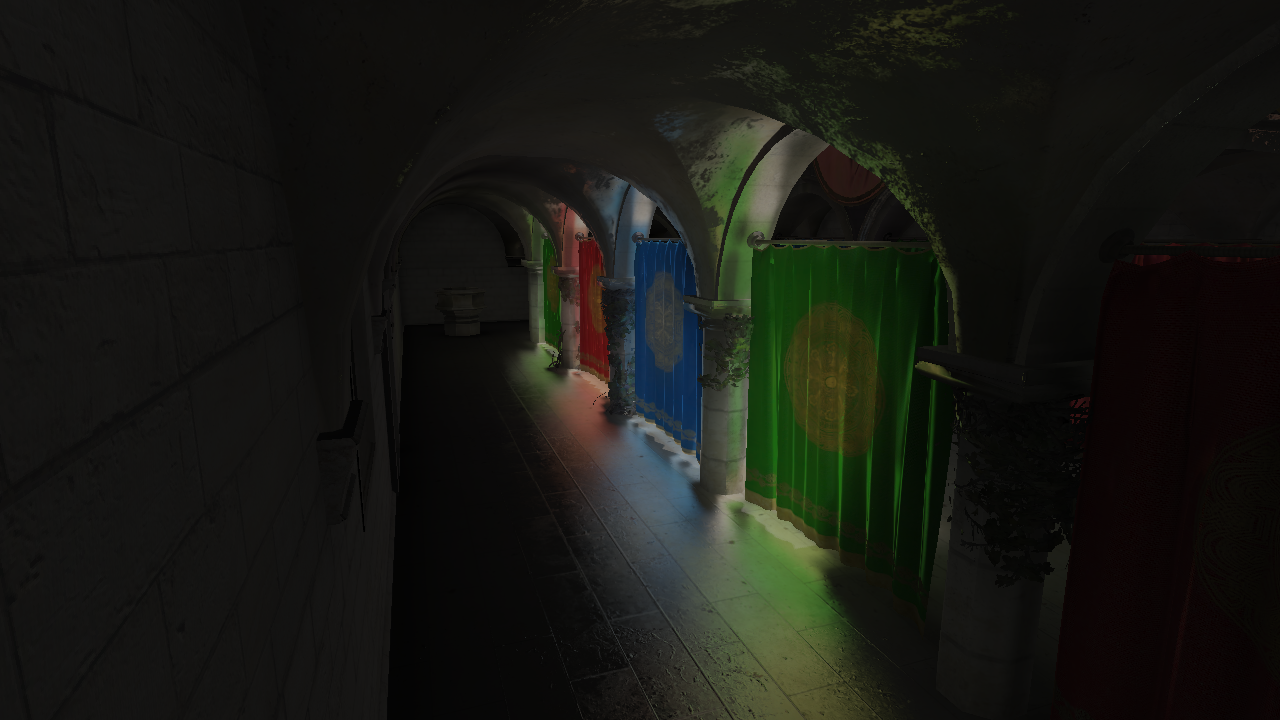
\includegraphics[width=\textwidth]{results_voxelraster.png}
        \caption{Rasterized voxels}
    \end{subfigure}
    ~
    \begin{subfigure}[t]{0.5\textwidth}
        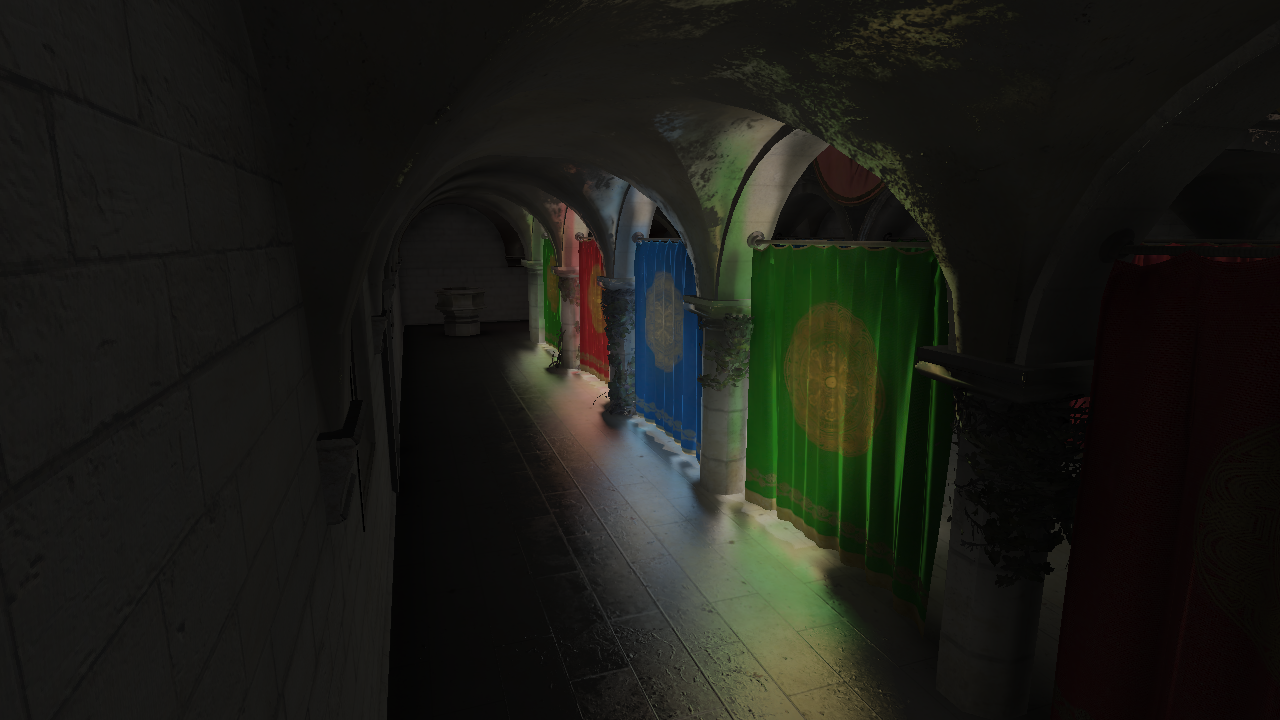
\includegraphics[width=\textwidth]{results_voxeltess.png}
        \caption{Tessellated voxels}
    \end{subfigure}
  \end{figure}

  \framebreak
  TODO table + graph

  % TODO have on their own slides too?
\end{frame}

% Lastly we evaluated our voxel warping...
\begin{frame}{Voxel Warping}
\end{frame}

{\setbeamertemplate{frame footer}{*Find the source here: \url{github.com/sfreed141/vct}}
\begin{frame}{Conclusion}
  % wrap up and list contributions again
\end{frame}}

\begin{frame}{Future Work}
  % other ways of adjusting resolution are more feasible due to temporal artifacts
  % spherical harmonics, directional filtering
  % grab bag of other optimizations related to voxel cone tracing
\end{frame}

\begin{frame}{}
  \begin{center}
    \LARGE Thank you!
  \end{center}
\end{frame}

\begin{frame}{}
  \begin{center}
    \LARGE Questions?
  \end{center}
\end{frame}

% TODO bibliography slides?

\section{Elements}

\begin{frame}[fragile]{Typography}
      \begin{verbatim}The theme provides sensible defaults to
\emph{emphasize} text, \alert{accent} parts
or show \textbf{bold} results.\end{verbatim}

  \begin{center}becomes\end{center}

  The theme provides sensible defaults to \emph{emphasize} text,
  \alert{accent} parts or show \textbf{bold} results.
\end{frame}

\begin{frame}{Font feature test}
  \begin{itemize}
    \item Regular
    \item \textit{Italic}
    \item \textsc{SmallCaps}
    \item \textbf{Bold}
    \item \textbf{\textit{Bold Italic}}
    \item \textbf{\textsc{Bold SmallCaps}}
    \item \texttt{Monospace}
    \item \texttt{\textit{Monospace Italic}}
    \item \texttt{\textbf{Monospace Bold}}
    \item \texttt{\textbf{\textit{Monospace Bold Italic}}}
  \end{itemize}
\end{frame}

\begin{frame}{Lists}
  \begin{columns}[T,onlytextwidth]
    \column{0.33\textwidth}
      Items
      \begin{itemize}
        \item Milk \item Eggs \item Potatos
      \end{itemize}

    \column{0.33\textwidth}
      Enumerations
      \begin{enumerate}
        \item First, \item Second and \item Last.
      \end{enumerate}

    \column{0.33\textwidth}
      Descriptions
      \begin{description}
        \item[PowerPoint] Meeh. \item[Beamer] Yeeeha.
      \end{description}
  \end{columns}
\end{frame}

\begin{frame}{Figures}
  \begin{figure}
    \newcounter{density}
    \setcounter{density}{20}
    \begin{tikzpicture}
      \def\couleur{alerted text.fg}
      \path[coordinate] (0,0)  coordinate(A)
                  ++( 90:5cm) coordinate(B)
                  ++(0:5cm) coordinate(C)
                  ++(-90:5cm) coordinate(D);
      \draw[fill=\couleur!\thedensity] (A) -- (B) -- (C) --(D) -- cycle;
      \foreach \x in {1,...,40}{%
          \pgfmathsetcounter{density}{\thedensity+20}
          \setcounter{density}{\thedensity}
          \path[coordinate] coordinate(X) at (A){};
          \path[coordinate] (A) -- (B) coordinate[pos=.10](A)
                              -- (C) coordinate[pos=.10](B)
                              -- (D) coordinate[pos=.10](C)
                              -- (X) coordinate[pos=.10](D);
          \draw[fill=\couleur!\thedensity] (A)--(B)--(C)-- (D) -- cycle;
      }
    \end{tikzpicture}
    \caption{Rotated square from
    \href{http://www.texample.net/tikz/examples/rotated-polygons/}{texample.net}.}
  \end{figure}
\end{frame}

\begin{frame}{Tables}
  \begin{table}
    \caption{Largest cities in the world (source: Wikipedia)}
    \begin{tabular}{lr}
      \toprule
      City & Population\\
      \midrule
      Mexico City & 20,116,842\\
      Shanghai & 19,210,000\\
      Peking & 15,796,450\\
      Istanbul & 14,160,467\\
      \bottomrule
    \end{tabular}
  \end{table}
\end{frame}

\begin{frame}{Blocks}
  Three different block environments are pre-defined and may be styled with an
  optional background color.

  \begin{columns}[T,onlytextwidth]
    \column{0.5\textwidth}
      \begin{block}{Default}
        Block content.
      \end{block}

      \begin{alertblock}{Alert}
        Block content.
      \end{alertblock}

      \begin{exampleblock}{Example}
        Block content.
      \end{exampleblock}

    \column{0.5\textwidth}

      \metroset{block=fill}

      \begin{block}{Default}
        Block content.
      \end{block}

      \begin{alertblock}{Alert}
        Block content.
      \end{alertblock}

      \begin{exampleblock}{Example}
        Block content.
      \end{exampleblock}

  \end{columns}
\end{frame}

\begin{frame}{Math}
  \begin{equation*}
    e = \lim_{n\to \infty} \left(1 + \frac{1}{n}\right)^n
  \end{equation*}
\end{frame}
\begin{frame}{Line plots}
  \begin{figure}
    \begin{tikzpicture}
      \begin{axis}[
        mlineplot,
        width=0.9\textwidth,
        height=6cm,
      ]

        \addplot {sin(deg(x))};
        \addplot+[samples=100] {sin(deg(2*x))};

      \end{axis}
    \end{tikzpicture}
  \end{figure}
\end{frame}

\begin{frame}{Bar charts}
  \begin{figure}
    \begin{tikzpicture}
      \begin{axis}[
        mbarplot,
        xlabel={Foo},
        ylabel={Bar},
        width=0.9\textwidth,
        height=6cm,
      ]

      \addplot plot coordinates {(1, 20) (2, 25) (3, 22.4) (4, 12.4)};
      \addplot plot coordinates {(1, 18) (2, 24) (3, 23.5) (4, 13.2)};
      \addplot plot coordinates {(1, 10) (2, 19) (3, 25) (4, 15.2)};

      \legend{lorem, ipsum, dolor}

      \end{axis}
    \end{tikzpicture}
  \end{figure}
\end{frame}

\begin{frame}{Quotes}
  \begin{quote}
    Veni, Vidi, Vici
  \end{quote}
\end{frame}

\begin{frame}{References}
  Some references to showcase [allowframebreaks] \cite{knuth92,ConcreteMath,Simpson,Er01,greenwade93}
\end{frame}

\appendix

\begin{frame}[fragile]{Backup slides}
  Sometimes, it is useful to add slides at the end of your presentation to
  refer to during audience questions.

  The best way to do this is to include the \verb|appendixnumberbeamer|
  package in your preamble and call \verb|\appendix| before your backup slides.

  \themename will automatically turn off slide numbering and progress bars for
  slides in the appendix.
\end{frame}

\begin{frame}[allowframebreaks]{References}

  \bibliography{demo}
  \bibliographystyle{abbrv}

\end{frame}

\end{document}
